% !TeX encoding = UTF-8
% !TeX spellcheck = es_ES
% !TeX root = Proto.tex
%!TEX root=Proto.tex
DccDiyTools es un repositorio de Módulos electrónicos, Objetos 3D y Documentación para la realización de maquetas
de Tren Digitales. En general los modulos se comunicaran usando protocolos estandard para este tipo de maquetas,
tales como DCC, Loconet, X-pressbus, C-Bus,… Y esto es correcto para los modulos individuales y completos que % chktex 8
interactúen con la maqueta. Pero hay veces que nos interesa partir estos modulos en componentes modulares o
simplemente debemos utilizar diferentes micro controladores para diferentes tareas y debemos poder comunicarnos
con todos los modulos.

\subsection{Modulo de Origen}
La idea de un protocolo de comunicaciones surge de una primera version de un panel de control de la maqueta.
Este panel básicamente es una caja donde en la tapa se ha pintado una versión esquemática de la maqueta y en las
posiciones de los desvíos se ha puesto unas palancas o interruptores y una cadena de leds WS2812 (usados tanto
para indicar el estado de los desvíos, como el estado de ocupación). El sistema se completa con dos interfaces,
una usb y otra LocoNet.

La idea original era usar un STM32 pero solo se disponía de un modelo con el que no se era capaz de usar los LEDS
(librerías del momento) y tampoco tenia suficientes pins para capturar los pulsos de los interruptores. Así que
se opto por usar 3 microcontroladores “básicos”, dos “Arduino” (“Atmega328”) y un stm32F103. Uno de los arduinos
se dejo para el bus LocoNet y la tira de leds y el otro para capturar los interruptores. Para comunicar se opto
por consultarlos periódicamente por I2C, puesto que requería pocos pines, siendo el STM32F103 el master y el que
coordina todo.

\subsection{Modulo de Ejemplo}
En el modulo anterior, el panel, en realidad la solución seria utilizar un micro controlador màs potente con más
pines, mas memoria y mas facilidades para multi-tarea. Y si bien podría ser un buen ejemplo para diseñar este % chktex 8
protocolo de comunicaciones vamos a centrarnos en una parte del Hobby que siempre ha sido la menos realista, y
nos aprovecharemos de otro Hobby que (gracias a las impresoras 3D) ha dado un gran impulso.

El modulo que vamos usar de modelo es un Panel de conducción más realista. Hoy por hoy los controles de velocidad
son una rueda que pone la velocidad del 0\% al 100\%. Hay diseños que la rueda es digital (una barra en una
pantalla) o se parece a un regulador de tranvia. Pero en cualquier caso se mantiene, a nivel de uso, el concepto
de un potenciomentro/rueda que controla el voltaje en la via.

Las maquinas de tren no funcionan asi, básicamente tienen 3 o 4 “palancas” teniendo su origen en las maquinas de
vapor:
\begin{itemize}
    \item{} Inversor, de tres posiciones, adelante, atrás o parada.
    \item{} Regulador, control de presión que va a los pistones (aceleración)
    \item{} Frenos, control de presión que va los frenos (frenos basicos)
\end{itemize}
La cuarta palanca son otros tipos de frenos (de vacío, del convoy,…). Además según modelos de tren puede haber palancas para los areneros, frenos dinámicos, silbatos,…

La excepción a todo esto el ProtoThrottle y nuestro modulo de ejemplo sera un panel realista de conducción. Diseño actual en desarrollo (20/07/2024):

\begin{figure}[H]
    \centering{}
    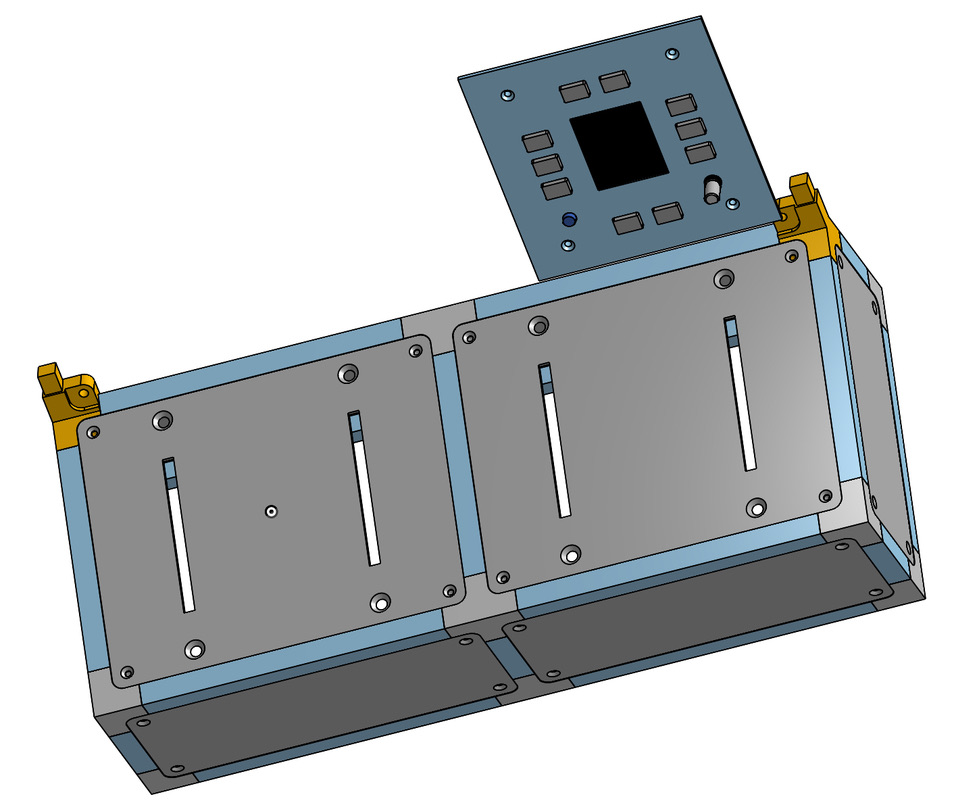
\includegraphics[scale=0.4]{images/EjemploEscritorio.jpeg}
    \caption{Ejemplo Escritorio Control}
    \label{fig:driverDeskExample}
\end{figure}
Figura 1 Ejemplo de panel en construccion
Este sistema tendrá que gestionar pantallas TFT, Palancas y Botones.

Como inspiración también se tiene la creación de cabinas personales de simulación de Avaviacion. En dicho hobby
se recrean cabinas muy realista, pero siempre se parte de la modularidad, esto es se divide en paneles
independientes, controlados cada uno con su arduino y este gestiona unos pocos botones/led para que sea realista.

En nuestro caso la idea es hacer diferentes paneles (TFT, Botones, dos o tres palancas,…) de tal forma que cada
uno se monte el panel como quiera y ajustado a sus necesidades.

Si no tenemos un protocolo de comunicaciones entre los paneles, necesitamos conectores específicos para cada tipo
de panel, por lo que el diseño de la placa central se complica y limita las posibilidades. Al añadir un protocolo
de comunicaciones podemos simplificar dicho diseño, pero implica un procesador por cada panel que transforme los
eventos del usuario a eventos del bus.

Así mismo no tiene sentido que cada panel se muestre al bus LCB emitiendo sus eventos y es mejor que se presente
al bus como un solo dispositivo y una placa central gestione cada panel.

\subsection{Problemas y Soluciones}
Además del problema obvio de pines (para capturar las pulsaciones de botones) el sistema inicial nos ha
identificado otros dos problemas, uno de ellos es la limitación de tiempo y coste de procesado, el otro es
la disponibilidad de librerías y/o periféricos.

\subsubsection{Detectar Pulsaciones}
El problema de capturar las pulsaciones de los botones de los usuarios es lineal, un botón -> un pin y ademas
nos interesa que sean interrupciones para que se capture la pulsación y no “haya” un coste computacional. Si no
son interrupciones debemos comprobar el estado del pin en cada bucle principal, pero esto implica que si el micro
procesador esta haciendo cosas largas, podamos perder pulsaciones por el usuario.

Las posibles soluciones son 4:
\begin{itemize}
    \item{} Uso de un procesador más poniente, con más pines e interrupciones.
    \item{} Matriz de MxN Keyboard  (\href{https://pcbheaven.com/wikipages/How_Key_Matrices_Works/}{How Key
              Matrices Works}) u otras variaciones basadas en resistencias/diodos. Esta solución require nos impide usar
          interrupciones y nos obliga a tener un bucle principal rápido y capturar el estado de los botones
    \item{} Usar un GPIO Expander o un chip de gestión de keyboard
    \item{} Usar un chip barato solo encargado de esto y usar un bus/protocolo propio
\end{itemize}

\subsubsection{Coste Computacional}
Ciertas operaciones requiren mucho tiempo de computación y si se realizan a la vez que el usuario interactúe con
el sistema es posible que se pierdan dichos eventos.

Por ejemplo el proceso de refrescar todos los leds WS2812 le lleva más de 100ms tiempo suficiente para que un
usuario pulse y libere un botón, si empezamos a añadir funciones, la ventana de oportunidad para detectar las
pulsaciones se reduce.

En este caso solo tenemos dos soluciones, o bien usamos un procesador más potente, bien usamos un procesador
para cada tarea intensiva.

\subsubsection{Disponibilidad de Librerías/Perifericos}
En el mercado existen diferentes micro-controladores que tienen periféricos diferentes como controladores CAN, % chktex 8
de LCD, WiFi, bluetooth y según las necesidad nos puede interesar usar uno u otro. En este caso de una forma u
otra deberemos acabar usando varios micro-controladores ya bien sea por usar varios con un bus controlado o con % chktex 8
chips dedicados y sus propios protocolos.

En este caso nos podemos encontrar con la (no) existencia de librerías para el micro elegido, con lo que usar
un bus propio nos permite tener chips que si nos lo soporte
